\section{Aspetti genrali}

\subsection{Analisi del nome}
Dal punto di vista sociale \`e fondamentale scegliere un buon nome per un
indirizzo web. Ci sono alcune regole che massimizzano il potenziale successo di
un sito. In media il 10-20\%, ma \`e possibile arrivare fino ad un +40-50\%
di influenza.

\textit{f1world.it} presenta delle buone caratteristiche a livello di nome,
infatti:
\begin{itemize}

\item \`e un nome corto, quindi risulta di facile memorizzazione per la maggior
  parte dell'utenza;
\item il nome risulta relativamente facile da memorizzare, in quanto composto
  da due parole (e facilmente memorizzabili anche per chi non parla inglese),
  \textit{f1} e \textit{world};
\item l'iniziale, essendo una \textit{f}, conferisce un bonus del +3.3\%;
\item all'interno dell'indirizzo \`e presente un numero, che conferisce un
  impatto bonus del +8.2\%.
\end{itemize}

A mio avviso il nome potrebbe aver avuto un impatto maggiore se avesse
utilizzato il dominio \textit{.com}.


\subsection{Elementi generali del sito web}

Di seguito verranno analizzati gli elementi in comune di tutto il sito web.
Viene presa come riferimento la homepage per questa analisi, ma pi\`u avanti
si far\`a un'analisi focalizzata solamente su di essa.

\begin{figure}[H]
  \centering
  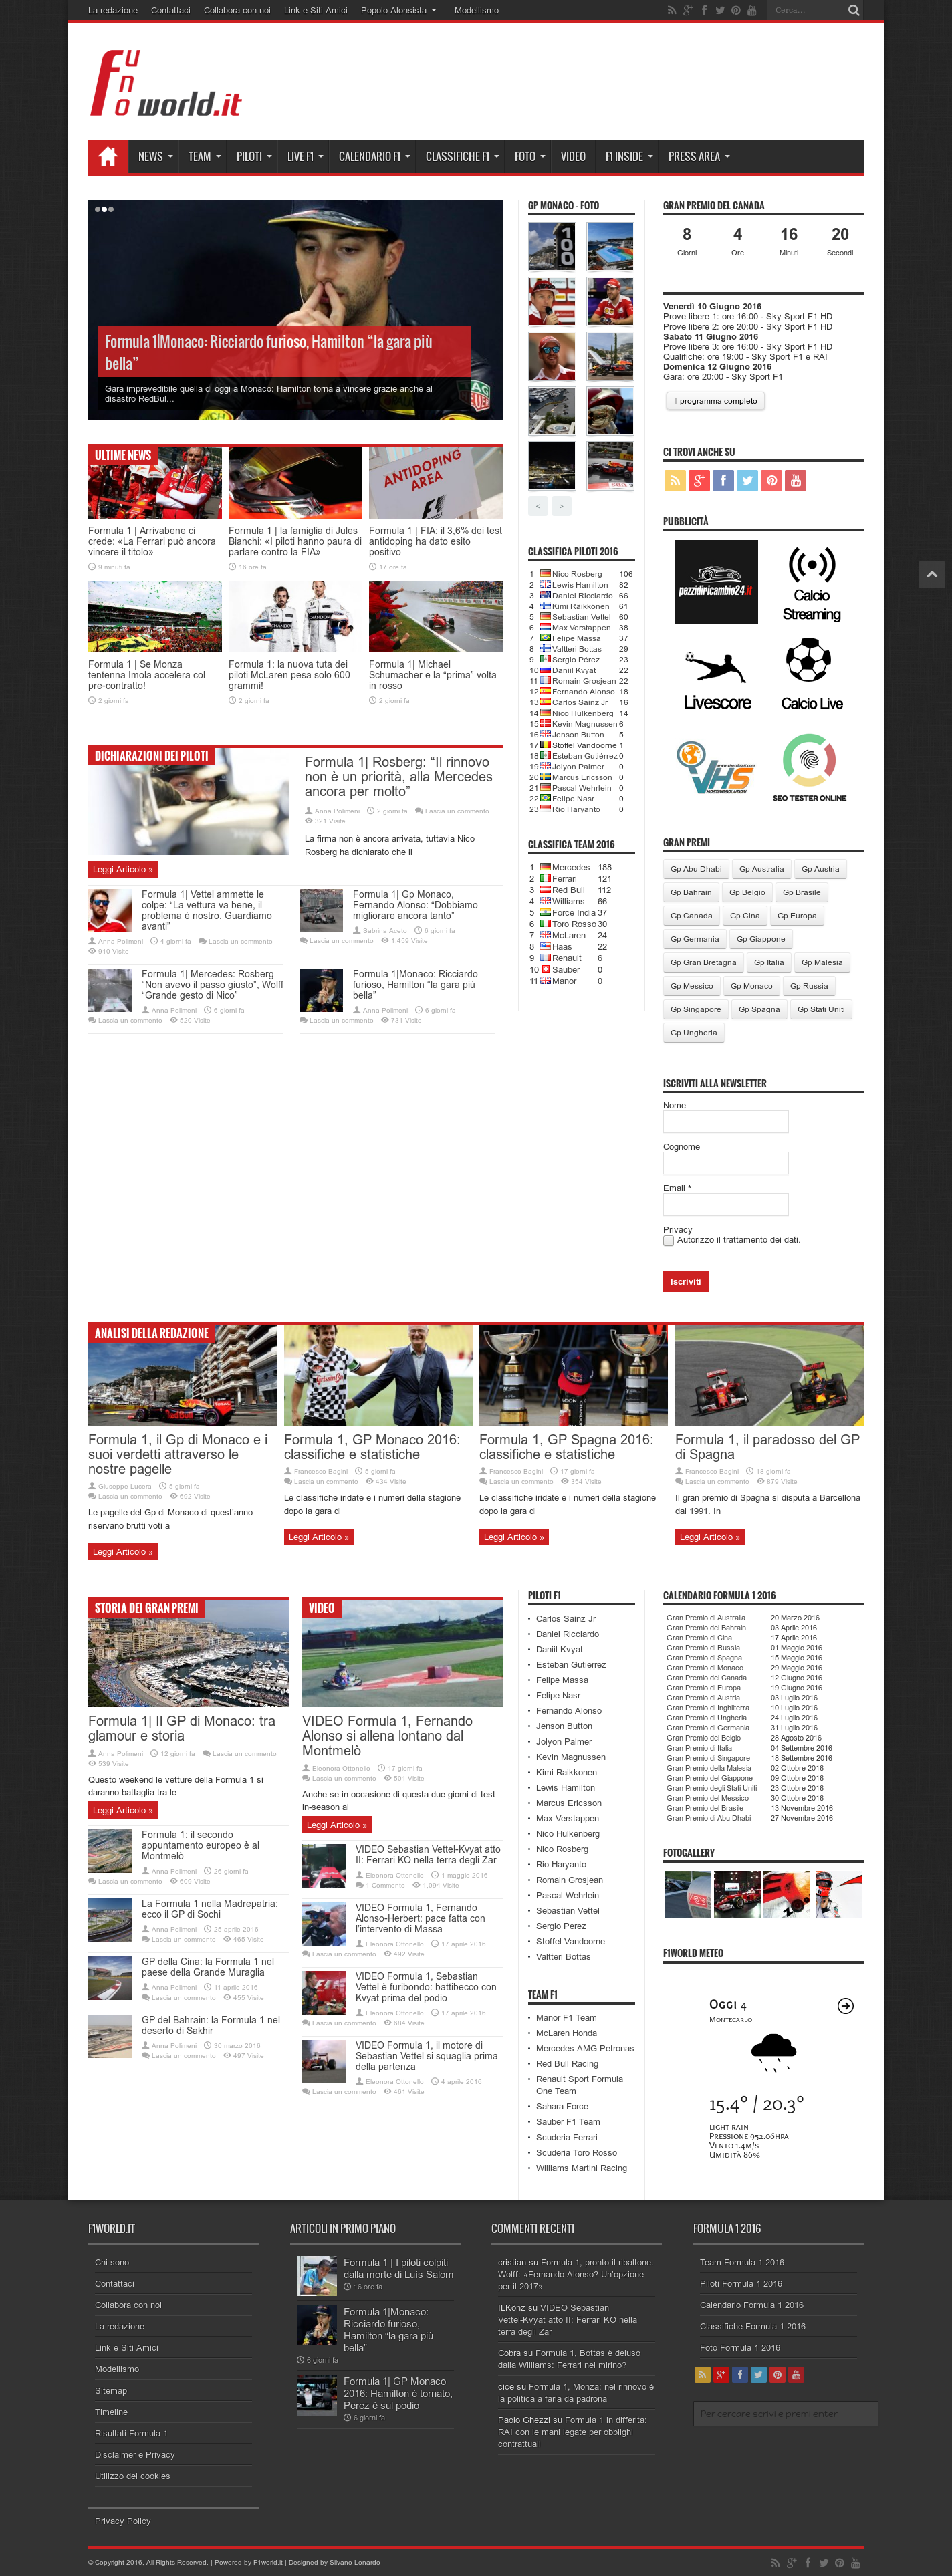
\includegraphics[height=18cm, width=10cm]{res/img/HomePage_Full}
  \caption{Homepage del sito, dove verranno analizzati solamente gli elementi
    che comuni a tutte le pagine.}
\end{figure}

L'analisi partir\`a dalla parte alta del sito per poi scendere fino in fondo.

\subsubsection{Header}

Come si pu\`o notare, all'inizio della pagina \`e presente un sottile header.
Nella sinistra dell'header troviamo dei link che ci portano a sezioni secondarie
rispetto ai temi trattati nel sito, mentre a destra troviamo delle icone per la
condivisione del sito web nei \textit{social network} e un box per la ricerca.
A mio avviso, questa disposizione degli elementi pu\`o essere migliorata. I link
presenti nella parte sinistra potrebbero essere spostati nella parte bassa del
sito web, per dare possibilit\`a alle icone di condivisione di essere spostate
sulla sinistra, lasciando quindi pi\`u spazio alla barra di ricerca, che in
questo modo diventerebbe pi\`u visibile all'utente e permetterebbe un migliore
inserimento della \textit{query} di ricerca. \`E infatti importante ricordare
come per una barra di ricerca sia importate lo spazio e la posizione: la
lunghezza media consigliata \`e di almeno 30 caratteri. Barre di ricerca troppo
piccole causano stress all'utente, che tendono a inserire \textit{query} di
ricerca pi\`u brevi diminuendo l'efficacia del motore di ricerca.


Subito sotto il piccolo header si trova il logo del sito web: questo logo
\`e composto da testo, il che aiuta l'utente a diminuire il senso di
disorientamento rispetto a un logo senza testo.
Accanto al logo \`e possibile notare uno spazio bianco, che a mio avviso
potrebbe essere riempito con del contenuto informativo.


Dopo il logo troviamo un men\`u orizzontale. Questo men\`u a tendina risulta
comodo per navigare nelle sezioni del sito: le voci si espandono al passaggio
del mouse (\textit{hover}), permettendo all'utente di eplorare comodamente i
sotto-argomenti trattati. Non \`e stato tenuto conto dell'algoritmo di
\textit{path finding} usato dall'utente per selezionare una delle varie voci: al
primo errore o alla prima fuoriuscita accidentale dal men\`u questo si chiude
subito, causandogli una forte irritazione che si trova
costretto a ripercorrere tutta la path svolta fino alla voce desiderata (si
ricorda che statisticamente il 92\% delle volte si esce dal cammino del men\`u).
Sarebbe meglio introdurre un men\`u \textit{fault-tolerant} che permetta
all'utente di non forzare il suo algoritmo di \textit{path finding}. Buono il
numero di livelli del men\`u che si ferma a due, rendendo meno impegnativa
l'esplorazione delle sotto-categorie.

\subsubsection{Corpo centrale}

Il sito web presenta un layout a tre colonne, dove nella colonna di sinistra si
trova sempre il contenuto della pagina richiesta (come ad esempio un articolo),
al centro si trova la colonna con le classifiche attuali del campionato e le
ultime foto presenti nel sito, e a destra sono presenti altre informazioni
secondarie. Questa distribuzione del contenuto fa richiedere un notevole sforzo
all'utente perch\`e viene utilizzato anche l'asse orizzontale per dare
l'informazione, riducendo lo spazio disponibile per il contenuto esplicitamente
richiesto da chi naviga. Sarebbe meglio ridurre il numero di colonne, per
aumentare la fruibilit\`a del sito.

\subsubsection{Footer}

Il footer ha un layout diviso in quattro colonne. La prima colonna a sinistra
presenta dei link a informazioni secondarie. Come si può ben notare, parte dei
link sono gli stessi di quelli che si trovano nell'header, causando quindi una
ripetizione che potrebbe portare confusione durante la navigazione.
Nella seconda colonna, troviamo una serie di articoli in ``primo piano''. La
posizione di questo elemento è poco consona alla sua posizione: come suggerito
dalle impronte termografiche sulle zone di visibilità di un
sito web, è possibile notare che il footer solitamente non rientra nella zona
``calda'' di visibilità degli utenti, e quindi questi articoli in ``primo piano''
non sono messi in risalto per un utente che naviga nel sito.
Nella terza colonna troviamo la lista degli articoli in cui sono stati scritti
di recente dei commenti dalla community, di cui non è possibile vederne
un'anteprima. Questo causa all'utente un possibile \textit{gambling click}
per visualizzare il commento.
L'ultima colonna riporta a delle risorse legate alla Formula1. Queste voci sono
in parte ripetute nel menù. Insieme a questi collegamenti è presente una serie
di icone per la condivisione e una seconda barra di ricerca (che risulta essere
poco intuitiva perchè manca del bottone ``search'' e/o di una icona della lente
di ricerca). Questa ripetizione di elementi, come già accennato prima, porta
disorientamento all'utente che viene messo in difficoltà da queste ripetizioni
dell'informazione.

\subsection{Distribuzione del testo e leggibilità}
%    - [ ] Text distribution and readability
Il sito web utilizza preventivamente tre tipi di colori, il nero il bianco e il
rosso, che vengono usati sapientemente in modo da avere sempre un buon risalto.
Vari colori vengono usati nelle seguenti situazioni:
\begin{itemize}

  \item il colore rosso costituisce una convenzione interna del sito in
  quando sta a indicare un \textit{link};

  \item il colore bianco viene usato per risaltare principalmente i titoli
  all'interno delle foto;

  \item il nero viene usato per il resto del testo.

\end{itemize}
Manca la possibilità di eseguire un \textit{resize} dei \textit{font}, dovendo
affidarsi al browser per questa funzionalità.
